\documentclass[11pt,a4paper,fontset=none]{ctexart}
\usepackage[margin=1in]{geometry}
\usepackage{fontspec}
% Latin: Times New Roman (Mac / Windows) or TeX Gyre Termes (Linux); CJK: Songti / Heiti (Mac) or Fandol by file name
\IfFontExistsTF{Times New Roman}{\setmainfont{Times New Roman}}{\setmainfont{TeX Gyre Termes}}
\IfFontExistsTF{Songti SC}{%
  \setCJKmainfont{Songti SC}[BoldFont={Songti SC Bold}]%
  \setCJKsansfont{Heiti SC}\setCJKmonofont{Heiti SC}}{%
  \setCJKmainfont{FandolSong-Regular.otf}[BoldFont=FandolSong-Bold.otf]%
  \setCJKsansfont{FandolHei-Regular.otf}[BoldFont=FandolHei-Bold.otf]\setCJKmonofont{FandolHei-Regular.otf}}
\usepackage{amsmath,amssymb}
\usepackage{booktabs,array,multirow,makecell,tabularx}
\usepackage{graphicx,float,adjustbox}
\usepackage[table]{xcolor}
\usepackage[font=small,labelfont=bf,labelsep=quad]{caption}
\usepackage{enumitem}
\usepackage[numbers,square,sort&compress]{natbib}
\usepackage{xurl}
\usepackage[colorlinks=true,linkcolor=blue!50!black,citecolor=green!40!black,urlcolor=blue!60!black]{hyperref}
\setlist{nosep,leftmargin=1.6em}
\ctexset{section={format=\Large\bfseries\raggedright},subsection={format=\large\bfseries\raggedright},
         abstractname=摘要}
\setlength{\parskip}{0.25em}
\renewcommand{\arraystretch}{1.12}
\newcommand{\ds}{DeepSeek Flash V4.1-1017}
\newcommand{\mini}{MiniMax M3.1 Flash}
\newcommand{\lead}[1]{\textbf{#1}\quad}
\pagestyle{plain}

\title{\textbf{codingBench：大模型代码能力评测基准}\\[0.3em]\large 技术报告}
\author{Albert Huang\\BAI AI Lab\\\small\url{https://github.com/BAI-AI-Lab/codingBench}}
\date{2026 年 10 月 31 日}

\begin{document}
\maketitle

\begin{abstract}
现有的代码评测正在迅速饱和：在 LiveCodeBench 最新的 35 道题上，复核判分后两个 DeepSeek 模型都做满 35 题，Kimi K3.1 Pro 做对 34 题，正确率已无法区分模型。而且，这些评测只看答案对不对，不看程序是否像人类选手一样在时限内跑完、用了什么复杂度的解法。本文提出 codingBench 阶梯评测：以人类竞赛的组别为难度标尺，从官方来源构建 L1--L5 五档、共 112 道题，其中 L1--L4 来自 USACO 2024--26 两个赛季的铜、银、金、铂金组与 EGOI 2026，L5 是没有已知最优解、按 0--100 连续计分的 FrontierCS 算法题。所有测试数据与参考解都来自官方发布，建库时先用官方解校验判题程序本身。每份答案在官方时限的 5 倍下只运行一次，同时得出“算法是否正确”（宽时限）与“能否在官方时限内通过”两种判定，并与官方解比较运行时间、内存与复杂度增长幂次；Python 档另报告静态代码质量。我们评测了 \ds 与 \mini：L1--L4 合计 pass@1 分别为 90.7\% 与 75.6\%，差 15.1 个百分点（按题配对 bootstrap 的 95\% 区间 9.9 至 20.9），差距随难度增大，在 L4 达到 22.2 个百分点；L5 两者分别为 30.6 与 25.6 分，差异不显著。只看官方时限时，两者在 L1、L2 上的 pass@1 相同。\mini 解出的答案平均更快、代码质量指标更好，但输出更长、更慢，总费用也更高。我们还把观测与两家厂商公开的技术声称逐条对照：\ds 在竞赛编程上的领先与其 Codeforces 评分的声称一致，\mini 所称的生成速度未能复现，两家关于智能体编程的声称不在本文的测量范围之内。代码与题号清单已开源。
\end{abstract}

\section{引言}

大模型写代码的能力进步很快，代码评测随之迅速饱和。我们此前用 LiveCodeBench~\cite{lcb} 最新发布的 35 道题评测了三个模型，复核判分后 DeepSeek-V4.1-Flash 与 DeepSeek-V4-Pro 都做对了全部 35 题，Kimi K3.1 Pro 做对 34 题；正确率已经无法区分它们，而同一批答案的运行时间却相差明显，相对最快答案的几何平均倍数在 1.29 至 2.74 之间。这说明现有评测至少有三个不足：

\begin{itemize}[leftmargin=1.6em]
  \item \lead{缺少难度梯度。}题目难度集中在一段，强模型很快做满，弱模型与强模型之间、强模型彼此之间都拉不开差距。
  \item \lead{只看对错。}答案能通过测试即算对，不论它是否在官方时限内跑完，也不论它用的是最优解法还是勉强通过的暴力解法。
  \item \lead{判分本身未经检验。}测试数据不全、比对规则过严或缺少多解 checker，都会把正确答案判错；我们在 LiveCodeBench 的复核中就遇到过这些问题。
\end{itemize}

为此我们构建了 codingBench 阶梯评测（图~\ref{fig:overview}）。它以人类竞赛的组别为难度标尺：USACO 的铜、银、金、铂金四个组别由真实选手的晋级线划定，EGOI 是国际奥赛，FrontierCS 收集的是没有已知最优解的开放问题。本文的主要贡献如下：

\begin{itemize}[leftmargin=1.6em]
  \item 我们给出一套按人类难度分为五档的竞赛编程题库，题目、测试数据与参考解全部来自官方发布，判题程序先用官方解校验，校验不通过的题一律剔除。
  \item 我们给出同时测正确性与效率的评测协议：一次运行同时得出宽时限与官方时限两种判定，并与官方解比较运行时间、内存与复杂度增长幂次；以按题配对的 bootstrap 与符号检验判断差距是否可信。
  \item 我们评测了 \ds 与 \mini，分析了它们在各档的正确率、两种时限的差别、新旧题对照、运行效率、失败类型、代码质量与成本，并把观测与厂商公开的技术声称逐条对照。
\end{itemize}

\begin{figure}[!tbp]
  \centering
  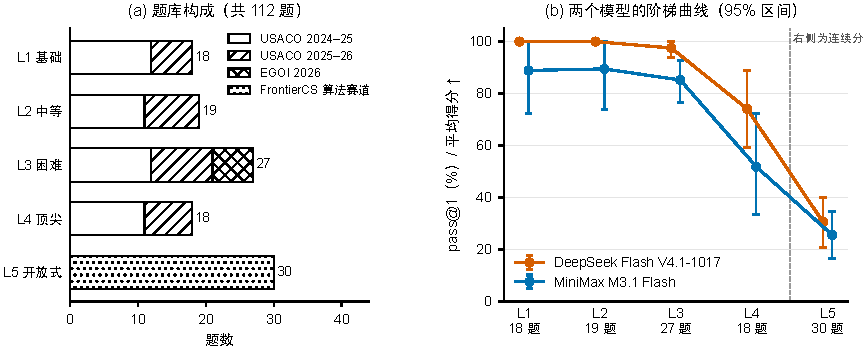
\includegraphics[width=\linewidth]{figures/fig1_overview.pdf}
  \caption{\textbf{codingBench 阶梯评测概览。}(a) 各档题数与来源，图案区分来源。(b) 两个模型在各档的主要指标与按题重抽样的 95\% 区间：L1--L4 为宽时限下的 pass@1，L5 为平均得分（连续分）。两个模型的差距从 L3 开始随难度增大，到 L5 又收窄。}
  \label{fig:overview}
\end{figure}

\section{相关工作}

\paragraph{正确性评测。}HumanEval~\cite{humaneval} 以函数级题目与 pass@$k$ 评测代码生成；APPS~\cite{apps} 与 AlphaCode 的 CodeContests~\cite{alphacode} 把评测扩展到竞赛题。为避免训练数据污染，LiveCodeBench~\cite{lcb} 持续收集新发布的竞赛题；USACO-Bench~\cite{usacobench} 使用 USACO 的历年题目，并按组别报告成绩。CodeElo~\cite{codeelo} 在 Codeforces 上提交并给出与人类可比的 Elo 分，LiveCodeBench Pro~\cite{lcbpro} 由奥赛奖牌得主标注题目难度与类型，OJBench~\cite{ojbench} 收集了 NOI、ICPC 等竞赛级题目。FrontierCS~\cite{frontiercs} 收集没有已知最优解的开放问题，按 checker 给出连续分。与这些工作相比，本文的题库只用官方的测试数据与参考解，并按人类组别分档，便于同时观察各难度段的差距。

\paragraph{效率与质量评测。}EffiBench~\cite{effibench} 与 ENAMEL~\cite{enamel} 比较生成代码与参考解的运行时间，Le 等人~\cite{perfbench} 讨论了性能评测本身的测量问题；BigO(Bench)~\cite{bigo} 通过规模扫描估计生成代码的时间与空间复杂度；AlgoTune~\cite{algotune} 评测模型能否加速数值程序。Huang 等人~\cite{quality} 用 Pylint、Radon 与 SonarQube 分析生成代码的静态质量，本文沿用其工具与版本。SWE-bench~\cite{swebench} 等仓库级、多轮的智能体编程评测考查的是另一种能力，不在本文范围之内。

\paragraph{统计方法。}我们以题目为重抽样单位，用 bootstrap~\cite{efron1979} 估计各档指标与两两差值的区间。

\section{阶梯基准}
\label{sec:bench}

\subsection{设计原则}

\begin{itemize}[leftmargin=1.6em]
  \item \lead{难度用人类标尺划分。}USACO 的四个组别由真实选手的晋级线划定，EGOI 是国际奥赛；档位反映的是人类选手的水平，而不是某个模型觉得难不难。
  \item \lead{只用官方数据。}AtCoder 自 2024 年 12 月起不再公开测试数据，LeetCode 的测试不公开且用户协议禁止批量抓取，这两个来源都给不出可信的标准答案，因此没有采用。
  \item \lead{高档用连续分。}USACO 按测试点给部分分，EGOI 按子任务给分，FrontierCS 由 checker 给出连续分，高档不会像通过率那样很快饱和。
  \item \lead{正确与速度分开测。}每个测试点只运行一次，时限放宽到官方的 5 倍，再按实际 CPU 时间同时得出两种判定：宽时限判的是算法对不对，官方时限判的是够不够快。
  \item \lead{先验证判题本身。}建库时先用我们的判题程序运行官方题解；没有任何一份官方解能全部通过的题直接剔除，这同时检验了测试数据、比对规则与判题程序。
\end{itemize}

\subsection{题库组成}

\begin{table}[!tbp]
  \centering
  \caption{\textbf{题库组成。}题数为最终进入评测的题数。USACO 每个组别计划 21 题，建库校验时剔除了没有官方解能通过、有多个合法答案却没有 checker 等无法可靠判分的题。}
  \label{tab:comp}
  \small
  \begin{tabularx}{\linewidth}{@{}l>{\raggedright\arraybackslash}Xrlll@{}}
    \toprule
    档位 & 来源 & 题数 & 比赛时间 & 作答语言 & 计分 \\
    \midrule
    L1 基础 & USACO 铜组 & 18 & 2024-12 至 2026-02 & Python & 测试点等分 \\
    L2 中等 & USACO 银组 & 19 & 2024-12 至 2026-02 & Python & 测试点等分 \\
    \multirow{2}{*}{L3 困难} & USACO 金组 & 21 & 2024-12 至 2026-02 & C++ & 测试点等分 \\
     & EGOI 2026（2026 子集） & 6 & 2026-05 & C++ & 子任务取最低分 \\
    L4 顶尖 & USACO 铂金组 & 18 & 2024-12 至 2026-02 & C++ & 测试点等分 \\
    L5 开放式 & FrontierCS 算法赛道（按题号均匀抽取） & 30 & 题库 v1.1 & C++17 & 0--100 连续分 \\
    \bottomrule
  \end{tabularx}
\end{table}

表~\ref{tab:comp} 给出了最终的题库组成，共 112 题。USACO~\cite{usaco} 取 2024--25 赛季的 12 月、1 月、2 月与美国公开赛共 4 场，以及 2025--26 赛季的 3 场线上赛（3 月的公开赛为线下监考赛，官网没有公布题目与测试数据）。EGOI 2026~\cite{egoi} 共 8 题，其中 Census 与 Seating Plan 是交互题，当前的判题程序不能正确评测，在评测后从题单中剔除，其答案不计入。计划中的 IOI 2026 题目本次没有纳入。FrontierCS~\cite{frontiercs,fcsrepo} 的题库有 180 道开放式难题，没有类别标签，我们按题号均匀抽取 30 题。题面与测试数据只存放在评测服务器上，不进入代码仓库；仓库只记录题号、档位、日期与时限。

\subsection{构建流程}

构建与评测流程如图~\ref{fig:pipeline} 所示。建库时，每道题的所有官方题解都要在全部测试点上判一遍：没有官方解能全部通过的题被剔除；能通过的官方解中最快的一份作为该题的性能对照。

\begin{figure}[!tbp]
  \centering
  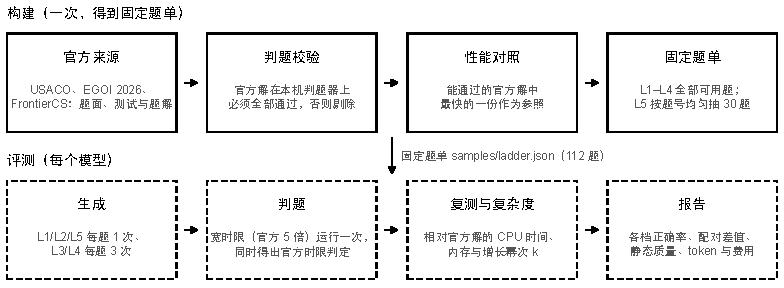
\includegraphics[width=\linewidth]{figures/fig2_pipeline.pdf}
  \caption{\textbf{构建与评测流程。}上行（实线框）只执行一次，得到固定题单；下行（虚线框）对每个模型执行，题目、判题程序与计分规则对所有模型完全相同。}
  \label{fig:pipeline}
\end{figure}

\section{判题、计分与统计方法}
\label{sec:method}

\subsection{运行环境与判定}

判题在评测服务器本机进行。答案以无特权用户运行，由一个小的启动器设置地址空间（内存上限加 64\,MB）、栈、CPU 时间与输出大小（256\,MB）上限，并把进程绑定在一个独占的核上；CPU 时间与峰值内存取自子进程自身的资源统计。Python 档使用 CPython 3.11、只允许标准库，官方时限沿用 USACO 给 Python 的时限；C++ 档以 \texttt{g++ -O2 -std=gnu++17} 编译。USACO 忽略空白逐个 token 比对，与其官方规则一致；EGOI 使用官方 checker；FrontierCS 使用官方的 testlib checker 或交互器，并照搬其判分规则，只解析 checker 输出的得分比例。

\subsection{计分}

每个测试点 $t$ 得分 $s_t \in [0, 1]$：编译失败、运行出错、超时或超内存记 0。每题得分 $S$（0--100）按来源的官方规则计算：USACO 为 $S = 100 \cdot \frac{1}{T}\sum_t s_t$；EGOI 为 $S = 100 \cdot \sum_g w_g \min_{t \in g} s_t / \sum_g w_g$，即子任务 $g$ 取其中测试点的最低分再乘以子任务分值；FrontierCS 为所有测试点得分比例的平均乘以 100，达到参考解约为 60 分，超过越多分越高。所有测试点都满分才算“解出”。

L1、L2、L5 每题采样 1 次，L3、L4 每题采样 3 次，以减小高档题少带来的随机误差。pass@1 是解出的采样占全部采样的比例，平均得分是全部采样的 $S$ 的平均，pass@$n$ 是至少有一次解出的题所占比例。L5 是连续分，只报告平均得分。

\subsection{宽时限与官方时限}

每个测试点只运行一次，时限为官方时限的 5 倍。宽时限口径按上述规则计分；官方时限口径把 CPU 时间超过官方时限的测试点记 0，再按同样的规则计分。前者回答“算法对不对”，后者回答“是否和人类选手一样在时限内通过”。

\subsection{运行效率与复杂度}

只对解出的答案、且官方解在某个测试点上至少需要 0.05 秒 CPU 的题比较运行时间：取官方解最慢的 3 个测试点，答案与官方解交替各运行 3 次取中位数，倍数为答案的 CPU 时间除以官方解的 CPU 时间，各档取几何平均。峰值内存倍数同理。

复杂度方面，官方测试并不是按规模排列的序列，USACO 中耗时可测的测试点几乎都是最大规模，直接按输入大小拟合基本不可行。因此我们以官方解自身的工作量为横轴：在官方解至少需要 2\,ms CPU 的测试点上（最多 20 个，均匀覆盖其耗时范围），答案与官方解交替各运行 5 次取中位数，拟合 $\log y_{\text{答案}} = a + k \log y_{\text{官方}}$。若官方解为 $\Theta(f(n))$、答案为 $\Theta(f(n)^k)$，$k$ 即为这个指数。只在拟合优度 $R^2 \ge 0.8$ 时下结论：$k \le 0.75$ 且在官方解最重的 3 个测试点上答案至少快 2 倍为更优，$0.75 < k < 1.33$ 为同阶，$k \ge 1.33$ 且至少慢 2 倍为更差，其余为不确定。

\subsection{静态代码质量}

对 L1、L2 中解出的 Python 答案，按 Huang 等人~\cite{quality} 的工具与版本，报告 Pylint 3.3.5 的问题数与 0--10 分，以及 Radon 6.0.1 的圈复杂度、可维护性指数（MI）与代码行数（SLOC）。SonarQube 需要 Docker，本次评测的机器上没有，未测。

\subsection{统计方法}

两个模型的比较以题目为单位。各档指标的 95\% 区间来自 $B = 2000$ 次按题重抽样：每次在每档内部有放回地抽取同样数量的题，重新计算各档与 L1--L4 合计的 pass@1 与平均得分，取 2.5\% 与 97.5\% 分位数；两个模型使用同一组题（配对 bootstrap），从而消除题目难度带来的共同波动。逐题比较取每题所有采样的平均得分，相差不到 0.05 分记为持平，并对胜负题数做精确符号检验。

\section{实验设置}
\label{sec:setup}

\subsection{被测模型}
\label{sec:models}

两个模型都是 2026 年 9--10 月发布的开放权重模型，都默认开启思考。下面依次概述它们的能力、厂商公开的技术要点及其所针对的能力，以及官方的代码评测成绩。以下内容来自厂商的技术博客、技术报告、模型卡与接口文档（访问于 2026 年 10 月 30 日），分数为厂商自报，未经独立复现。

\paragraph{\ds。}DeepSeek 于 2026 年 9 月 10 日发布 V4.1-Flash，10 月 17 日更新为 1017 版，接口名与价格不变，以 MIT 许可开放权重~\cite{ds1017}。模型为多模态 MoE，主干 552B 参数、每 token 激活 8B（prefill）/ 16B（decode），另有 196B 的 Engram 条件记忆，上下文 1M。技术报告~\cite{dsv41} 的主要创新在注意力与 KV cache 的压缩，面向长上下文与“输入很重”的智能体场景的服务成本；报告明确说后训练“没有算法上的创新”，沿用监督微调、强化学习与在线蒸馏的标准流程，改动都在数据上，并在训练中按思考深度施加长度惩罚，使深度可调。报告称其 Codeforces 评分（内部评测）为 3471，高于 V4-Flash 的 3289 与 V4-Pro 的 3348。1017 版称以自反馈强化学习改进端到端的项目开发，并缩短了任务耗时与输出长度；厂商自报（智能体框架）Terminal-Bench 4.0 由 31.2 提高到 42.3、DeepSWE v1.1 由 74.2 提高到 77.0、ProgramBench 由 20.3 提高到 29.1~\cite{ds1017}。官方评测使用最高思考深度，而接口默认的深度为 high~\cite{dsapi}。

\paragraph{\mini。}MiniMax 于 2026 年 10 月 19 日上线接口、10 月 23 日开放权重；MoE 架构，总参数约 428B、每 token 激活约 23B，上下文 1M，思考不能关闭，默认最高深度~\cite{minimaxm31}。厂商称 M3.1 Flash 沿用前代 M3 的核心架构，只做了三处改动：全部层改为稀疏注意力，路由专家与注意力路径做量化感知训练，以 DSpark 投机解码代替原先的多 token 预测。这三处都面向推理速度与成本：官方称输出速度可达每秒 200 token 以上、中位数稳定在 170 以上，在线推理快近 3 倍、使用成本降低 70\%。厂商把它定位于智能体任务，称其原生支持在每轮工具调用之间思考（交错思考），自报 DeepSWE v1.1 73.7、Terminal Bench 4.0 38.1、NL2Repo-Bench 61.2~\cite{minimaxm31}；前代 M3 自报 SWE-Bench Verified 80.5~\cite{minimaxm3}。两家都没有报告与本文题源重合的竞赛编程评测（如 LiveCodeBench、USACO、IOI 或 FrontierCS），\mini 也没有报告任何竞赛编程成绩。

\subsection{调用设置}

两个模型都通过各自厂商的官方接口流式调用（表~\ref{tab:models}），temperature 为 0.2、top\_p 为 0.95（沿用 LiveCodeBench 的设置；DeepSeek 在思考模式下不支持 temperature 参数~\cite{dsapi}），输出上限 262,144 token。两个模型都没有设置思考深度，即使用接口默认值：\mini 默认为最高档，\ds 默认为 high，低于其官方评测所用的最高档。因此本文 \ds 的成绩可能低于它在最高深度下的水平。单次生成超过 20 分钟即被切断：\mini 有 13 个采样被切断，以 30 分钟为限重问一次后 3 个完成、10 个仍未完成（其中 6 个是服务端在约 24--30 分钟时主动断开），记为“生成超时”；\ds 没有调用超过 20 分钟。被切断的请求没有用量返回，其输出 token 按已输出的字数估算。提示词见附录~\ref{app:prompts}。

\begin{table}[!tbp]
  \centering
  \caption{\textbf{被测模型与调用设置。}单价为各厂商的公开标价（美元 / 百万 token），依次为输入（缓存未命中）、缓存命中与输出；\ds 在北京时间非高峰时段半价，费用按每次调用的开始时间计算。}
  \label{tab:models}
  \small
  \begin{adjustbox}{max width=\linewidth}
  \begin{tabular}{llccc}
    \toprule
    模型 & API 名称 & 思考深度 & 输出上限 & 单价（输入 / 缓存命中 / 输出） \\
    \midrule
    \ds & \texttt{deepseek-flash} & 接口默认（high） & 262,144 & 0.30 / 0.006 / 1.20（非高峰半价） \\
    \mini & \texttt{MiniMax-M3.1-Flash} & 接口默认（max） & 262,144 & 0.15 / 0.015 / 0.60 \\
    \bottomrule
  \end{tabular}
  \end{adjustbox}
\end{table}

\subsection{归因规则}
\label{sec:attr-rule}

厂商声称的改进大多相对其上一代模型而言，而本文只评测了两个不同的模型，没有评测它们的前代，因此无法检验“是否比前代更好”。我们检验较弱的命题：厂商声称擅长或改进的方向，在本文对应的测量上是否表现为显著的相对优势。一条声称同时满足以下两点时，记为\textbf{一致，可归因}：
\begin{itemize}[leftmargin=1.6em]
  \item 厂商指明了它针对的能力，且能对应到本文的某个档位或某项测量（正确率、运行效率、生成速度、输出长度等）；
  \item 在这项测量上，该模型相对另一个模型的差值显著（区间不含 0），方向与声称一致；对于可直接测量的绝对数值（如生成速度），本文的测量值与声称相符。
\end{itemize}
方向相反或测量值与声称不符时记为\textbf{不一致}；对应不到本文测量的声称（如多轮的智能体编程）记为\textbf{本文未测}；只是相对前代的数量声称，记为\textbf{无法检验}；观测到明显差异但没有对应声称的，记为\textbf{无对应声称}，不作归因。这种归因只说明观测与声称不矛盾，而不是因果：两个模型在数据、规模与训练方法上同时不同，本文没有消融实验。

\section{实验结果}

\subsection{主要结果}

表~\ref{tab:main} 与图~\ref{fig:scores} 给出了两个模型在各档的正确率。

\begin{table}[!tbp]
  \centering
  \caption{\textbf{各档正确率（越高越好 $\uparrow$）。}每行两个模型中较高者加粗；灰色为按题重抽样的 95\% 区间（L1--L4 为宽时限 pass@1，L5 为平均得分）。L1、L2、L5 每题采样 1 次，没有 pass@$n$；L5 为连续分，没有 pass@1。合计行的 pass@1 按采样数加权。}
  \label{tab:main}
  \small
  \setlength{\tabcolsep}{4.5pt}
  \begin{adjustbox}{max width=\linewidth}\begin{tabular}{llrrrrrrrr}
\toprule
 & & & & \multicolumn{2}{c}{pass@1（\%）$\uparrow$} & \multicolumn{2}{c}{平均得分 $\uparrow$} & & \\
\cmidrule(lr){5-6}\cmidrule(lr){7-8}
档位 & 模型 & 题数 & 采样数 & 宽时限 & 官方时限 & 宽时限 & 官方时限 & pass@$n$（\%）$\uparrow$ & 95\% 区间 \\
\midrule
\multirow{2}{*}{L1 基础} & DeepSeek & 18 & 18 & \textbf{100.0} & 83.3 & \textbf{100.0} & \textbf{94.7} & -- & {\scriptsize\color{gray}100.0--100.0} \\
 & MiniMax & 18 & 18 & 88.9 & 83.3 & 89.4 & 88.5 & -- & {\scriptsize\color{gray}72.2--100.0} \\
\midrule
\multirow{2}{*}{L2 中等} & DeepSeek & 19 & 19 & \textbf{100.0} & 84.2 & \textbf{100.0} & \textbf{95.2} & -- & {\scriptsize\color{gray}100.0--100.0} \\
 & MiniMax & 19 & 19 & 89.5 & 84.2 & 89.8 & 87.0 & -- & {\scriptsize\color{gray}73.7--100.0} \\
\midrule
\multirow{2}{*}{L3 困难} & DeepSeek & 27 & 81 & \textbf{97.5} & \textbf{96.3} & \textbf{98.3} & \textbf{98.3} & 100.0 & {\scriptsize\color{gray}93.8--100.0} \\
 & MiniMax & 27 & 81 & 85.2 & 85.2 & 88.1 & 88.1 & 100.0 & {\scriptsize\color{gray}76.5--92.6} \\
\midrule
\multirow{2}{*}{L4 顶尖} & DeepSeek & 18 & 54 & \textbf{74.1} & \textbf{72.2} & \textbf{77.2} & \textbf{76.6} & \textbf{94.4} & {\scriptsize\color{gray}59.3--88.9} \\
 & MiniMax & 18 & 54 & 51.9 & 51.9 & 55.1 & 55.1 & 72.2 & {\scriptsize\color{gray}33.3--72.2} \\
\midrule
\multirow{2}{*}{L5 开放式} & DeepSeek & 30 & 30 & -- & -- & \textbf{30.6} & \textbf{28.6} & -- & {\scriptsize\color{gray}20.7--40.0} \\
 & MiniMax & 30 & 30 & -- & -- & 25.6 & 24.5 & -- & {\scriptsize\color{gray}16.4--34.5} \\
\midrule
\multirow{2}{*}{L1--L4 合计} & DeepSeek & 82 & 172 & \textbf{90.7} & \textbf{86.0} & -- & -- & -- & {\scriptsize\color{gray}85.5--95.9} \\
 & MiniMax & 82 & 172 & 75.6 & 74.4 & -- & -- & -- & {\scriptsize\color{gray}68.0--83.1} \\
\bottomrule
\end{tabular}
\end{adjustbox}
\end{table}

\begin{figure}[!tbp]
  \centering
  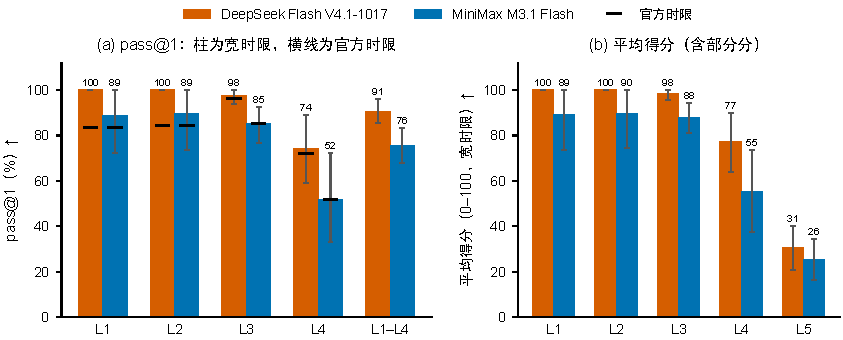
\includegraphics[width=\linewidth]{figures/fig3_scores.pdf}
  \caption{\textbf{各档正确率与 95\% 区间。}(a) 柱为宽时限下的 pass@1，黑色横线为官方时限下的 pass@1；(b) 平均得分（含部分分）。}
  \label{fig:scores}
\end{figure}

\lead{\ds 在每一档都领先，差距在 L3、L4 显著。}L1--L4 合计，\ds 的 pass@1 为 90.7\%，\mini 为 75.6\%，差 15.1 个百分点（配对区间 9.9 至 20.9）。逐题比较（112 题），\ds 更好 39 题、\mini 更好 9 题、持平 64 题，符号检验 $p < 0.001$。分档看（表~\ref{tab:pairwise}，图~\ref{fig:pairwise}），L1、L2 的差距各只来自 2 道题，区间包含 0；L3 差 12.3 个百分点、L4 差 22.2 个百分点，区间都不含 0。L4 的 18 道题中有 12 道 \ds 更好，没有一道 \mini 更好；按至少一次解出计，\ds 解出 94.4\% 的题，\mini 为 72.2\%。

\lead{开放式的 L5 两者都远未饱和，差距不显著。}L5 平均得分 \ds 为 30.6，\mini 为 25.6，差 5.0 分（区间 $-3.4$ 至 13.1），逐题 14 比 8、持平 8，$p = 0.29$。FrontierCS 达到参考解约为 60 分，两个模型的平均水平都低于参考解。

\begin{table}[!tbp]
  \centering
  \caption{\textbf{逐档配对比较。}差值为 \mini 减去 \ds，负数表示 \ds 更高；$^{*}$ 表示配对 bootstrap 的 95\% 区间不含 0。逐题比较取每题所有采样的平均得分，相差不到 0.05 分记为持平。}
  \label{tab:pairwise}
  \small
  \begin{adjustbox}{max width=\linewidth}\begin{tabular}{lrrrrrr}
\toprule
 & \multicolumn{2}{c}{pass@1 差（百分点）} & \multicolumn{2}{c}{平均得分差} & & \\
\cmidrule(lr){2-3}\cmidrule(lr){4-5}
档位 & 差值 & 95\% 区间 & 差值 & 95\% 区间 & 逐题 DeepSeek 更好 / 持平 / MiniMax 更好 & 符号检验 $p$ \\
\midrule
L1 基础 & $-$11.1 & [$-$27.8, +0.0] & $-$10.6 & [$-$26.3, +0.0] & 2 / 16 / 0 & 0.500 \\
L2 中等 & $-$10.5 & [$-$26.3, +0.0] & $-$10.2 & [$-$25.7, +0.0] & 2 / 17 / 0 & 0.500 \\
L3 困难 & $-$12.3$^{*}$ & [$-$21.0, $-$4.9] & $-$10.2$^{*}$ & [$-$17.6, $-$4.3] & 9 / 17 / 1 & 0.021 \\
L4 顶尖 & $-$22.2$^{*}$ & [$-$33.3, $-$11.1] & $-$22.1$^{*}$ & [$-$32.3, $-$12.5] & 12 / 6 / 0 & $<0.001$ \\
L5 开放式 & -- & -- & $-$5.0 & [$-$13.1, +3.4] & 14 / 8 / 8 & 0.286 \\
\midrule
L1--L4 合计 & $-$15.1$^{*}$ & [$-$20.9, $-$9.9] & $-$12.9$^{*}$ & [$-$18.3, $-$7.7] & 25 / 56 / 1 & $<0.001$ \\
\bottomrule
\end{tabular}
\end{adjustbox}
\end{table}

\begin{figure}[!tbp]
  \centering
  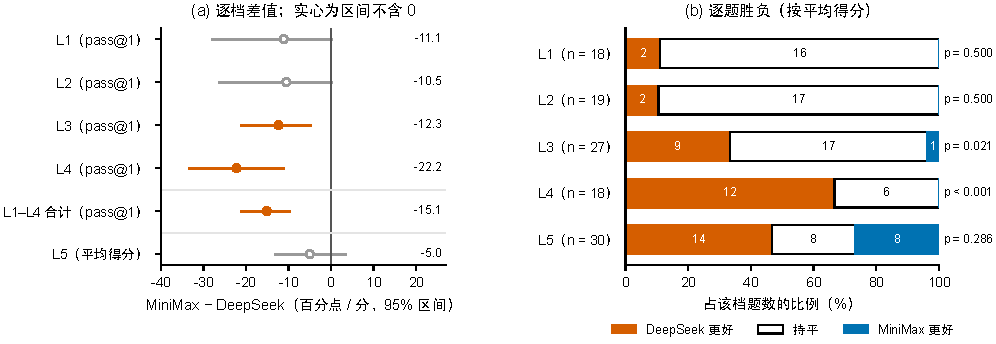
\includegraphics[width=\linewidth]{figures/fig4_pairwise.pdf}
  \caption{\textbf{逐档比较。}(a) 点为差值，横线为配对 bootstrap 的 95\% 区间，实心表示区间不含 0；(b) 逐题胜负，柱内数字为题数，右侧为符号检验的 $p$ 值。}
  \label{fig:pairwise}
\end{figure}

\subsection{只看官方时限，差距在哪里？}

在 Python 作答的 L1、L2 上，两种时限的差别最明显。\ds 在宽时限下解出了 L1、L2 的全部题目，但各有 3 道题的答案只在宽时限下通过，运行时间超过了官方时限，官方时限下的 pass@1 降为 83.3\% 与 84.2\%；\mini 在这两档各有 1 道这样的题，官方时限下同样是 83.3\% 与 84.2\%，但两者解出的题并不完全相同。也就是说，\ds 在 Python 档的优势在于把算法写对，而它的 Python 答案更常超出官方时限；按人类选手的规则判，两者在这两档的 pass@1 相同。C++ 作答的 L3、L4 几乎不受影响，官方时限下 \ds 仍分别领先 11.1 与 20.3 个百分点（表~\ref{tab:main}）。

\subsection{新题是否明显更难？}

题目可能出现在模型的训练数据中。表~\ref{tab:subsets} 把同一档内的 2026 年新题与 USACO 旧题分开统计。L3 中 EGOI 2026 的 6 道新题上，\ds 全部解出，\mini 为 83.3\%，都与各自在同档 USACO 旧题上的成绩相近（\ds 96.3\%--97.2\%，\mini 85.2\%--86.1\%），没有显示旧题成绩被训练数据明显抬高的迹象。L4 只有 USACO 题，其中较新的 2025--26 赛季上，\mini 的 pass@1 只有 33.3\%，远低于它在 2024--25 赛季上的 63.6\%，\ds 则分别为 71.4\% 与 75.8\%。这一差别只有 7 道题、且两个赛季的难度分布不完全相同，只能作为提示，不能作为结论。

\begin{table}[!tbp]
  \centering
  \caption{\textbf{2026 年新题与 USACO 旧题的对照（宽时限）。}每格两个模型中较高者加粗。}
  \label{tab:subsets}
  \small
  \begin{adjustbox}{max width=\linewidth}\begin{tabular}{llrrrrr}
\toprule
 & & & \multicolumn{2}{c}{pass@1（\%，宽时限）$\uparrow$} & \multicolumn{2}{c}{平均得分 $\uparrow$} \\
\cmidrule(lr){4-5}\cmidrule(lr){6-7}
档位 & 子集 & 题数 & DeepSeek & MiniMax & DeepSeek & MiniMax \\
\midrule
L3 困难 & EGOI 2026（新题） & 6 & \textbf{100.0} & 83.3 & \textbf{100.0} & 84.4 \\
L3 困难 & USACO 2024--25 & 12 & \textbf{97.2} & 86.1 & \textbf{98.8} & 89.2 \\
L3 困难 & USACO 2025--26 & 9 & \textbf{96.3} & 85.2 & \textbf{96.6} & 89.1 \\
L4 顶尖 & USACO 2024--25 & 11 & \textbf{75.8} & 63.6 & \textbf{78.4} & 64.7 \\
L4 顶尖 & USACO 2025--26 & 7 & \textbf{71.4} & 33.3 & \textbf{75.3} & 40.2 \\
\bottomrule
\end{tabular}
\end{adjustbox}
\end{table}

\subsection{解出的答案有多快？}

表~\ref{tab:eff} 与图~\ref{fig:eff} 只比较解出的答案。两个模型的答案在各档都比官方解快：\ds 为官方解 CPU 时间的 0.58 至 0.96 倍，\mini 为 0.42 至 0.55 倍。在 L4 上，\ds 有 9 份答案比官方解慢 2 倍以上，\mini 只有 2 份。复杂度方面，绝大多数可判定的答案与官方解同阶；\mini 有更多答案被判为增长更慢（L3 上 11 份，\ds 为 4 份），这些答案已单独列出、待人工复核。需要注意的是，两个模型解出的题并不相同：\mini 解出的题更少，若它更多地解出较容易、较易写出快速解法的题，这一比较会偏向它。

\begin{table}[!tbp]
  \centering
  \caption{\textbf{解出答案的运行效率与时间复杂度（相对官方解，同语言）。}倍数小于 1 表示比官方解快或省内存；只比较官方解在某个测试点上至少需要 0.05 秒 CPU 的题。EGOI 与 FrontierCS 没有可用作对照的官方解，不参与。}
  \label{tab:eff}
  \small
  \begin{adjustbox}{max width=\linewidth}\begin{tabular}{llrrrrrl}
\toprule
档位 & 模型 & 比较的答案数 & CPU 时间倍数 $\downarrow$ & 快于官方解 & 慢 2 倍以上 & 峰值内存倍数 $\downarrow$ & 时间复杂度：更优 / 同阶 / 更差 / 不确定 \\
\midrule
\multirow{2}{*}{L1 基础} & DeepSeek & 12 & 0.66$\times$ & 10 & 2 & 0.98$\times$ & 1 / 4 / 0 / 3 \\
 & MiniMax & 10 & 0.42$\times$ & 9 & 1 & 0.80$\times$ & 3 / 3 / 0 / 3 \\
\midrule
\multirow{2}{*}{L2 中等} & DeepSeek & 9 & 0.84$\times$ & 7 & 0 & 1.32$\times$ & 0 / 6 / 0 / 0 \\
 & MiniMax & 8 & 0.54$\times$ & 8 & 0 & 1.14$\times$ & 0 / 6 / 0 / 0 \\
\midrule
\multirow{2}{*}{L3 困难} & DeepSeek & 58 & 0.58$\times$ & 47 & 3 & 0.92$\times$ & 4 / 42 / 2 / 10 \\
 & MiniMax & 51 & 0.45$\times$ & 43 & 0 & 0.83$\times$ & 11 / 35 / 0 / 8 \\
\midrule
\multirow{2}{*}{L4 顶尖} & DeepSeek & 37 & 0.96$\times$ & 18 & 9 & 1.25$\times$ & 4 / 28 / 0 / 1 \\
 & MiniMax & 25 & 0.55$\times$ & 21 & 2 & 0.99$\times$ & 3 / 19 / 1 / 0 \\
\bottomrule
\end{tabular}
\end{adjustbox}
\end{table}

\begin{figure}[!tbp]
  \centering
  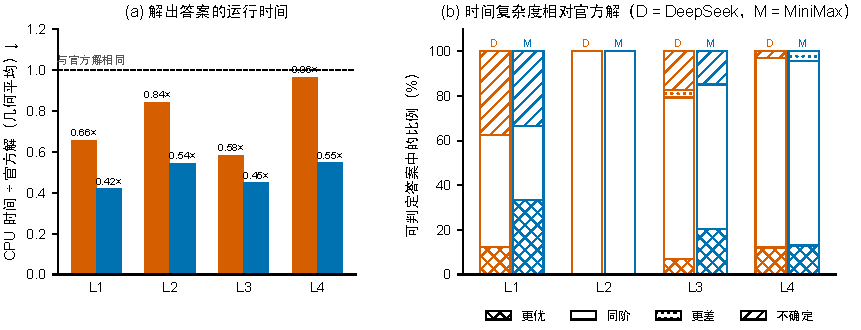
\includegraphics[width=\linewidth]{figures/fig5_efficiency.pdf}
  \caption{\textbf{运行效率与复杂度。}(a) 解出答案的 CPU 时间相对官方解的几何平均，虚线为与官方解相同；(b) 时间复杂度判定的构成，边框颜色区分模型，图案区分判定。}
  \label{fig:eff}
\end{figure}

\subsection{答案为什么没有解出？}

表~\ref{tab:fail} 给出每份答案的主要失败原因。\ds 在 L1--L4 的失败几乎全是答案错误，集中在 L4（12 份）。\mini 的失败更分散：L4 上有 7 份生成超时、6 份编译错误、11 份答案错误，L5 上有 7 份编译错误。生成超时与编译错误这两类失败与算法能力无关，若能消除，\mini 在 L4 上的差距会缩小一部分。

\begin{table}[!tbp]
  \centering
  \caption{\textbf{失败类型（答案数）。}每份答案只记一个主要原因。“只在官方时限下超时”的答案在宽时限下是解出的，单独列出。L5 为连续分，得分大于 0 的答案记为部分分。}
  \label{tab:fail}
  \small
  \begin{adjustbox}{max width=\linewidth}\begin{tabular}{ll*{9}{r}}
\toprule
档位 & 模型 & 答案数 & 无代码 & 生成超时 & 编译错误 & 答案错误 & 部分分 & 运行错误 & 超时 & 只在官方时限下超时 \\
\midrule
\multirow{2}{*}{L1 基础} & DeepSeek & 18 & 0 & 0 & 0 & 0 & 0 & 0 & 0 & 3 \\
 & MiniMax & 18 & 0 & 0 & 0 & 1 & 0 & 1 & 0 & 1 \\
\midrule
\multirow{2}{*}{L2 中等} & DeepSeek & 19 & 0 & 0 & 0 & 0 & 0 & 0 & 0 & 3 \\
 & MiniMax & 19 & 0 & 0 & 0 & 2 & 0 & 0 & 0 & 1 \\
\midrule
\multirow{2}{*}{L3 困难} & DeepSeek & 81 & 0 & 0 & 0 & 2 & 0 & 0 & 0 & 1 \\
 & MiniMax & 81 & 0 & 0 & 3 & 9 & 0 & 0 & 0 & 0 \\
\midrule
\multirow{2}{*}{L4 顶尖} & DeepSeek & 54 & 1 & 0 & 0 & 12 & 0 & 1 & 0 & 1 \\
 & MiniMax & 54 & 2 & 7 & 6 & 11 & 0 & 0 & 0 & 0 \\
\midrule
\multirow{2}{*}{L5 开放式} & DeepSeek & 30 & 2 & 0 & 1 & 4 & 23 & 0 & 0 & 0 \\
 & MiniMax & 30 & 0 & 1 & 7 & 3 & 17 & 0 & 2 & 0 \\
\bottomrule
\end{tabular}
\end{adjustbox}
\end{table}

\subsection{代码质量}

表~\ref{tab:quality} 只统计 L1、L2 中解出的 Python 答案。\mini 的答案更短（平均 54.4 行，\ds 为 67.1 行），Pylint 问题更少（每百行 9.1 个，\ds 为 13.0 个），圈复杂度更低、可维护性指数更高。两者的 Pylint 得分都在 8.6 分以上。

\begin{table}[!tbp]
  \centering
  \caption{\textbf{静态代码质量（L1、L2 中解出的 Python 答案，每份平均）。}较好者加粗；SLOC 只作描述。}
  \label{tab:quality}
  \small
  \begin{adjustbox}{max width=\linewidth}\begin{tabular}{l*{7}{r}}
\toprule
模型 & 答案数 & Pylint 问题数 $\downarrow$ & Pylint 得分 $\uparrow$ & 每百行问题数 $\downarrow$ & 圈复杂度 $\downarrow$ & 可维护性 MI $\uparrow$ & SLOC \\
\midrule
DeepSeek Flash V4.1-1017 & 37 & 8.73 & 8.68 & 13.01 & 19.03 & 51.2 & 67.1 \\
MiniMax M3.1 Flash & 33 & \textbf{4.97} & \textbf{8.98} & \textbf{9.13} & \textbf{14.67} & \textbf{62.4} & 54.4 \\
\bottomrule
\end{tabular}
\end{adjustbox}
\end{table}

\subsection{观测到的差异能否归因于厂商声称的技术改进？}
\label{sec:attr}

表~\ref{tab:attr} 按第~\ref{sec:attr-rule} 节的规则，把第~\ref{sec:models} 节列出的技术声称与本文的观测逐条对照。

\begin{table}[!tbp]
  \centering
  \caption{\textbf{厂商声称与本文观测的对照。}差值为 \ds 减去 \mini，方括号内为配对 bootstrap 的 95\% 区间；“一致”只表示观测与声称不矛盾，不表示因果。}
  \label{tab:attr}
  \footnotesize
  \renewcommand{\arraystretch}{1.05}\setlength{\tabcolsep}{4pt}
  \begin{tabularx}{\linewidth}{@{}>{\raggedright\arraybackslash}p{4.3cm}>{\raggedright\arraybackslash}p{1.7cm}>{\raggedright\arraybackslash}X>{\raggedright\arraybackslash}p{2.3cm}@{}}
\toprule
厂商声称 & 对应维度 & 本文观测（DeepSeek $-$ MiniMax，95\% 区间） & 判定 \\
\midrule
\multicolumn{4}{@{}l}{\textbf{DeepSeek Flash V4.1-1017}} \\
Codeforces 评分 3471（内部评测，max 深度），高于 V4-Flash 的 3289 与 V4-Pro 的 3348 & 竞赛编程 & pass@1 领先 MiniMax：L1--L4 合计 +15.1 [+9.9, +20.9]，L3 +12.3 [+4.9, +21.0]，L4 +22.2 [+11.1, +33.3] & 一致，可归因（相对 MiniMax） \\
1017 版以自反馈强化学习改进端到端项目开发；智能体编程（DeepSWE v1.1 77.0、Terminal-Bench 4.0 42.3） & 多轮、多文件编程 & 本文为单轮、单文件、无工具的作答 & 本文未测 \\
1017 版缩短输出长度与任务耗时（相对 0910 版） & — & 每次调用平均输出 42.3k token，短于 MiniMax 的 58.6k；没有 0910 版对照 & 无法检验 \\
按思考深度施加长度惩罚、深度可调 & 思考深度 & 本文使用接口默认的 high，未比较不同深度 & 本文未测 \\
\midrule
\multicolumn{4}{@{}l}{\textbf{MiniMax M3.1 Flash}} \\
推理速度：输出可达每秒 200 token 以上、中位数 170 以上 & 生成速度 & 首个 token 之后的平均生成速度 116 token/s，低于所称；DeepSeek 为 177 & 不一致（国内站、8 路并发） \\
智能体编程与工具调用（DeepSWE v1.1 73.7、Terminal Bench 4.0 38.1）；交错思考 & 多轮、多文件编程 & 本文为单轮、单文件、无工具的作答 & 本文未测 \\
在线推理快近 3 倍、使用成本降低 70\%（相对前代） & — & 没有前代对照；本文费用 \$7.58，高于 DeepSeek 的 \$6.07 & 无法检验 \\
没有竞赛编程方面的声称或成绩 & 竞赛编程 & L3、L4 的 pass@1 均显著落后 DeepSeek（见上） & 无对应声称 \\
\bottomrule
\end{tabularx}

\end{table}

\lead{竞赛编程上的领先与 \ds 的声称一致。}\ds 的技术报告以 Codeforces 评分（内部评测 3471）作为核心推理能力的证据，\mini 没有报告任何竞赛编程成绩；本文中 \ds 在 L3、L4 与 L1--L4 合计上都显著领先，与之一致。值得注意的是，本文 \ds 使用的是接口默认的 high 深度，低于其官方评测的最高深度，它的领先并不依赖最高深度。

\lead{智能体编程的声称不在本文的测量范围内。}两家的主要宣传都放在多轮、带工具的智能体编程上（DeepSWE、Terminal-Bench 等），而本文是单轮、单文件、不带工具的竞赛编程。\mini 在本文的落后并不与它在智能体编程上的声称矛盾。

\lead{效率方面的声称多数无法检验，可检验的一条未能复现。}\mini 称输出速度中位数稳定在每秒 170 token 以上；本文测得它在首个 token 之后的平均生成速度为每秒 116 token，低于所称，也低于 \ds 的 177。本文通过国内站、8 路并发调用，这些条件可能拉低速度；被切断的超时请求按字数估算 token，也会带来误差。\ds 1017 版“缩短输出长度”的声称是相对 0910 版而言，本文没有前代对照，无法检验；本文中它每次调用平均输出 42.3k token，确实短于 \mini 的 58.6k。

\section{成本与 token 效率}
\label{sec:cost}

表~\ref{tab:usage} 与图~\ref{fig:cost} 给出了各档的用量与费用。尽管 \mini 的输出单价只有 \ds 高峰价的一半，它的总费用（7.58 美元）仍高于 \ds（6.07 美元），每份解出答案的费用为 0.045 美元，\ds 为 0.031 美元。原因是 \mini 每次调用的输出更长（平均 58.6k token，\ds 为 42.3k），解出的题又更少；而 \ds 的调用多在非高峰时段，实际按半价计费。两者的延迟差距更大：\mini 每次调用的延迟中位数为 350 秒，\ds 为 177 秒；在 L4 与 L5 上，\mini 的延迟中位数分别为 12.3 与 14.2 分钟。思考在输出中所占的比例，\ds 为 97.2\%，\mini 为 72.7\%。

\begin{table}[!tbp]
  \centering
  \caption{\textbf{各档用量与费用（越低越好 $\downarrow$）。}输出 token 含思考；每份解出答案的费用为该档费用除以宽时限下解出的采样数，合计只算 L1--L4。\mini 的 L4、L5 调用数含超时后的重问。\ds 合计中另含 6 次对已剔除题的调用（0.28 美元）。}
  \label{tab:usage}
  \small
  \begin{adjustbox}{max width=\linewidth}\begin{tabular}{llrrrrrr}
\toprule
档位 & 模型 & 调用数 & 输出 token $\downarrow$ & 每次输出 $\downarrow$ & 延迟中位数（秒）$\downarrow$ & 费用 $\downarrow$ & 每份解出答案 $\downarrow$ \\
\midrule
\multirow{2}{*}{L1 基础} & DeepSeek & 18 & 0.18M & 10.0k & 49 & \$0.11 & \$0.006 \\
 & MiniMax & 18 & 0.27M & 15.0k & 64 & \$0.16 & \$0.010 \\
\midrule
\multirow{2}{*}{L2 中等} & DeepSeek & 19 & 0.48M & 25.2k & 106 & \$0.29 & \$0.015 \\
 & MiniMax & 19 & 0.75M & 39.6k & 194 & \$0.45 & \$0.027 \\
\midrule
\multirow{2}{*}{L3 困难} & DeepSeek & 81 & 2.41M & 29.7k & 126 & \$1.45 & \$0.018 \\
 & MiniMax & 81 & 2.95M & 36.4k & 200 & \$1.78 & \$0.026 \\
\midrule
\multirow{2}{*}{L4 顶尖} & DeepSeek & 54 & 3.71M & 68.6k & 398 & \$3.01 & \$0.075 \\
 & MiniMax & 64 & 5.81M & 90.7k & 739 & \$3.49 & \$0.125 \\
\midrule
\multirow{2}{*}{L5 开放式} & DeepSeek & 30 & 1.55M & 51.8k & 233 & \$0.94 & -- \\
 & MiniMax & 33 & 2.82M & 85.5k & 853 & \$1.70 & -- \\
\midrule
\multirow{2}{*}{合计} & DeepSeek & 208 & 8.80M & 42.3k & 177 & \$6.07 & \$0.031 \\
 & MiniMax & 215 & 12.60M & 58.6k & 350 & \$7.58 & \$0.045 \\
\bottomrule
\end{tabular}
\end{adjustbox}
\end{table}

\begin{figure}[!tbp]
  \centering
  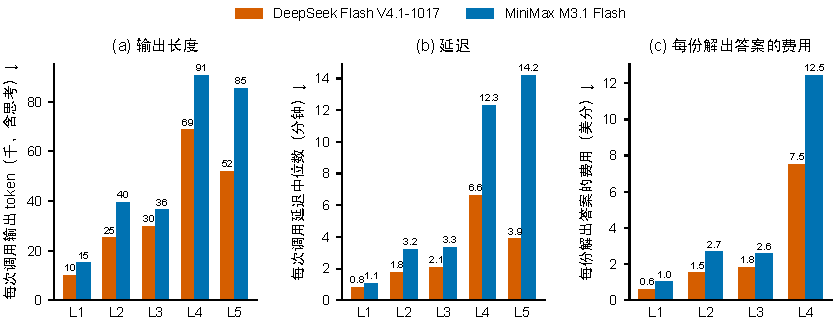
\includegraphics[width=\linewidth]{figures/fig6_cost.pdf}
  \caption{\textbf{成本与速度。}(a) 每次调用的平均输出 token（含思考）；(b) 每次调用的延迟中位数；(c) 每份解出答案的费用。均为越低越好。}
  \label{fig:cost}
\end{figure}

\section{结论}

我们提出了 codingBench 阶梯评测：以人类竞赛组别为难度标尺，从官方来源构建五档、112 道题，一次运行同时给出宽时限与官方时限下的正确性，并与官方解比较运行效率与复杂度。对两个开放权重模型的评测表明，\ds 的领先从 L3 开始随难度扩大，在 L4 达到 22 个百分点，与其在竞赛编程上的声称一致；而在 L1、L2 上，它的 Python 答案更常超出官方时限，按官方时限计两者的 pass@1 相同。\mini 解出的答案更快、代码更简洁，但输出更长、更慢，总费用也更高。两个模型在开放式的 L5 上都远低于参考解，这一档仍有很大的区分空间。这些归因都是观测上的一致，确认因果仍需对照实验。后续工作包括：评测更多模型（包括 Kimi K3.1 Pro），支持交互题与 IOI 的通信题，以及为 USACO 编写输入生成器，做真正的规模扫描。

\section*{局限性}

\begin{itemize}[leftmargin=1.6em]
  \item \lead{只评测了两个模型。}本文没有在阶梯评测上评测 Kimi K3.1 Pro 等更多模型，模型之间的相对位置只在这两个模型之间成立。
  \item \lead{思考深度不对等。}两个模型都使用接口默认的思考深度：\mini 为最高档，\ds 为 high。\ds 在最高深度下的成绩可能更高。
  \item \lead{归因是观测上的一致，而非因果。}两个模型在数据、规模与训练方法上同时不同，本文既没有消融实验，也没有评测它们的前代。
  \item \lead{题目覆盖不全。}EGOI 的 2 道交互题在评测后剔除，IOI 2026 的题目没有纳入；高档题量少，L3、L4 只有 27 与 18 题，区间较宽。
  \item \lead{题目时效。}USACO 题目截至 2026 年 2 月，可能已进入部分模型的训练数据；2026 子集的对照只能作为提示。
  \item \lead{效率比较存在选择偏差。}运行效率与代码质量只比较各自解出的答案，两个模型解出的题并不相同。
  \item \lead{费用与速度受调用条件影响。}费用按公开标价计算，不代表实际支出；生成速度受并发与网络条件影响，被切断请求的 token 为估算值。
\end{itemize}

\bibliographystyle{unsrtnat}
\bibliography{refs}

\appendix
\section{提示词}
\label{app:prompts}

USACO 与 EGOI 题沿用 LiveCodeBench 的写法，并给出时限与内存限制；FrontierCS 使用其官方生成脚本的原始提示词，便于与其公开排行榜对照。系统提示词与格式说明如下（原文为英文）：

{\raggedright\small
\begin{itemize}[leftmargin=1.6em]
  \item Python 档系统提示词：\texttt{You are an expert Python programmer. You will be given a question (problem specification) and will generate a correct Python program that matches the specification and passes all tests.}
  \item C++ 档系统提示词：\texttt{You are an expert competitive programmer. You will be given a question (problem specification) and will generate a correct and efficient C++17 program that matches the specification and passes all tests.}
  \item 用户消息：\texttt{\#\#\# Question:} 之后为题面，随后一行写明时限、内存限制与语言（如 \texttt{Time limit: 2 seconds per test. Memory limit: 256 MB. Compiled with g++ -O2 -std=gnu++17.}），再给出格式说明：\texttt{Read the inputs from stdin solve the problem and write the answer to stdout (do not directly test on the sample inputs). Enclose your code within delimiters as follows.}
  \item FrontierCS：\texttt{You are a competitive programmer. You will be given a problem statement, please implement a solution in C++. The execution time and memory limit are also stated in the statement so be aware of the complexity of the program. Please wrap the code in \textasciigrave\textasciigrave\textasciigrave cpp and \textasciigrave\textasciigrave\textasciigrave{} so that it is properly formatted. Your response should ONLY contain the C++ code, with no additional explanation or text.}
\end{itemize}
\par}

答案取回答中最后一个对应语言的代码块（LiveCodeBench 的规则），没有对应语言时取最后一个代码块。

\section{复现}
\label{app:repro}

代码、题单生成脚本与本文的全部图表脚本见 \url{https://github.com/BAI-AI-Lab/codingBench}。题面、测试数据与官方题解不随仓库发布，需从官方来源重新下载（\texttt{cb ladder-data}）并建库：

\begin{small}
\begin{verbatim}
cb ladder-data                 # 下载官方数据（可断点续传）
cb ladder-build --calibrate    # 整理题目，判官方解并选出性能对照
export MODEL=... OPENAI_BASE_URL=... OPENAI_API_KEY=...
cb ladder --smoke              # 每档 1 题，先确认接口
cb ladder                      # 生成、判题、性能复测、复杂度、静态质量、报告
cb ladder-report <运行A> <运行B> --out <目录>
\end{verbatim}
\end{small}

本文的数字、表格与图由仓库 \texttt{paper} 目录下的三个脚本从已提交的运行报告（\nolinkurl{reports/2026-10-29_ladder_deepseek-flash_vs_minimax-m3.1-flash/report.json}）生成：\texttt{analysis.py} 计算统计量，\texttt{make\_tables.py} 生成表格，\texttt{make\_figures.py} 绘图。

\vspace{2em}\begin{flushright}由 Albert Huang 创建于 2026-10-31\end{flushright}

\end{document}
